\chapter{Activation Functions}\label{chapter: Activation Functions}

\section{Definition \cite{wiki-Artificial_neuron, wiki-activation-fn}}

The activation function of a node in an artificial neural network is a function that calculates the output of the node based on its individual inputs and their weights. Nontrivial problems can be solved using only a few nodes if the activation function is nonlinear

\vspace{0.2cm}
\begin{itemize}
    \item  The transfer functions usually have a \textbf{sigmoid} shape, but they may also take the form of other non-linear functions, piecewise linear functions, or step functions.
    \item They are also often monotonically increasing, continuous, differentiable and bounded. 
    \item  Non-monotonic, unbounded and oscillating activation functions with multiple zeros that outperform sigmoidal and ReLU-like activation functions on many tasks have also been recently explored
\end{itemize}

\vspace{0.2cm}
\noindent From \cite{wiki-Artificial_neuron} \\

\begin{itemize}
    \item $n$ is number of inputs
    \item $w_i$ is a vector of synaptic weights
    \item $x_i$ is a vector of inputs
\end{itemize}
\[
    u=\sum _{i=1}^{n}w_{i}x_{i}
\]

$u$ refers in all cases to the weighted sum of all the inputs to the neuron

\section{Step function \cite{wiki-Artificial_neuron}}\label{Step function}

\begin{figure}[H]
    \centering
    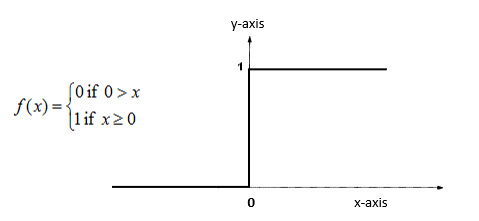
\includegraphics[height=3cm]{Pictures/activation-fns/step-function.jpg}
    \caption{Activation Function: Step Function}
\end{figure}

\[
    y={\begin{cases}1&{\text{if }}u\geq \theta \\0&{\text{if }}u<\theta \end{cases}}
\]

\begin{itemize}
    \item The output y of this transfer function is binary, depending on whether the input meets a specified threshold, $\theta$. 
    \item The "signal" is sent, i.e. the output is set to one, if the activation meets the threshold.
    \item It performs a division of the space of inputs by a hyperplane. 
    \item It is specially useful in the last layer of a network intended to perform binary classification of the inputs. 
    \item It can be approximated from other sigmoidal functions by assigning large values to the weights.
\end{itemize}


\section{Linear combination \cite{wiki-Artificial_neuron}}
\[
    y = u + b
\]

\begin{itemize}
    \item The output unit is simply the weighted sum of its inputs plus a bias term. A number of such linear neurons perform a linear transformation of the input vector. 
    \item This is usually more useful in the first layers of a network. 
    \item A number of analysis tools exist based on linear models, such as harmonic analysis, and they can all be used in neural networks with this linear neuron. 
    \item The bias term allows us to make affine transformations to the data.
\end{itemize}



\section{Sigmoid function \cite{wiki-activation-fn,wiki-Sigmoid_function}}

\begin{itemize}
    \item A sigmoid function is any mathematical function whose graph has a characteristic S-shaped or sigmoid curve.
    \item A sigmoid function is a bounded, differentiable, real function that is defined for all real input values and has a non-negative derivative at each point and exactly one inflection point.
    \item A sigmoid function is monotonic, and has a first derivative which is bell shaped
    \item The integral of any continuous, non-negative, bell-shaped function (with one local maximum and no local minimum, unless degenerate) will be \textbf{sigmoidal}.
    \item A sigmoid function is constrained by a pair of \textbf{horizontal asymptotes} as $x\rightarrow \pm \infty$
    \item A sigmoid function is \textbf{convex} for values less than a particular point, and it is \textbf{concave} for values greater than that point: in many of the examples here, that point is 0.
\end{itemize}

\subsection{Logistic function ( $\sigma(x)$ ) \cite{wiki-Logistic_function,wiki-Sigmoid_function}}\label{Logistic function}

\begin{figure}[H]
    \centering
    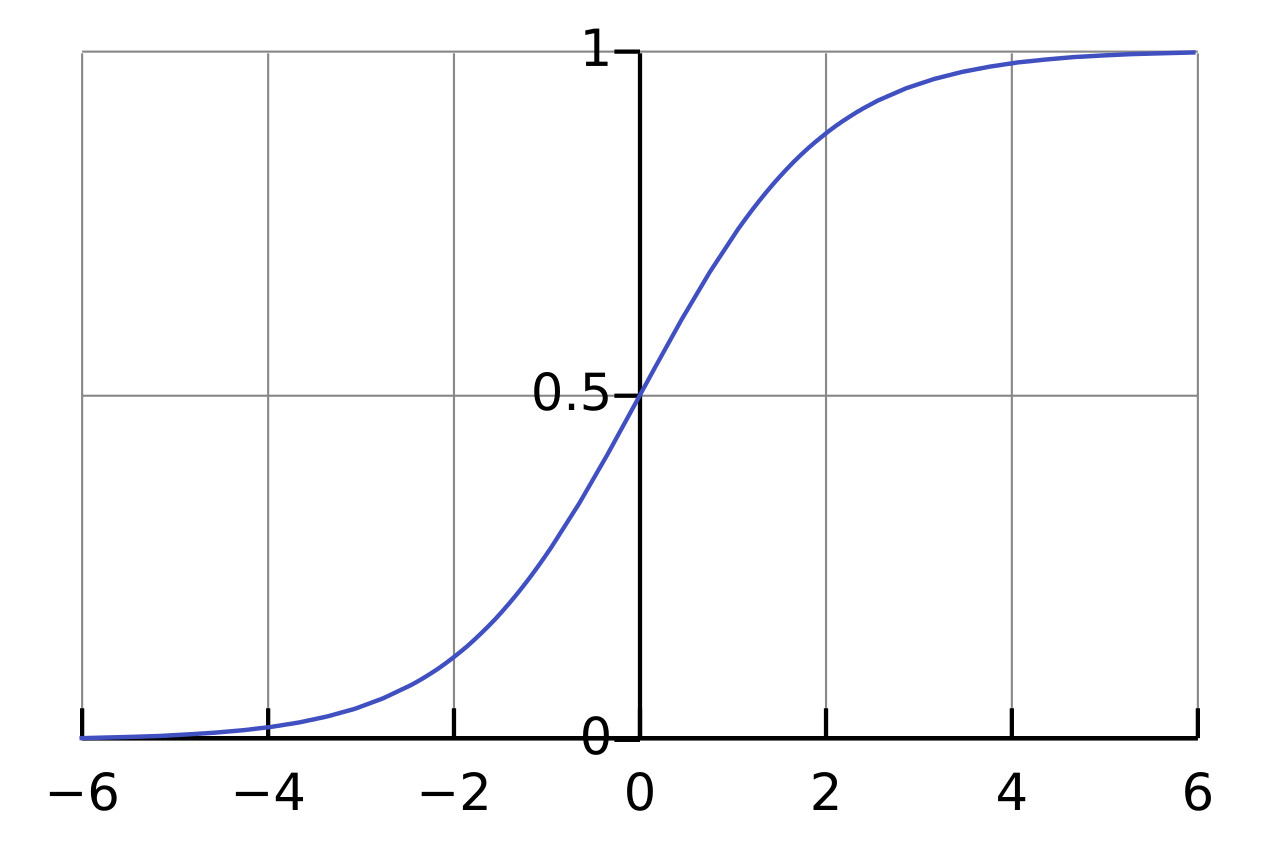
\includegraphics[height=3cm]{Pictures/activation-fns/sigmoid-fn.jpg}
    \caption{Activation Function: Sigmoid Function}
\end{figure}

General Equation:
\[
    f(x) = {\displaystyle\dfrac{L}{1 + e^{-k(x - x_{0})}}}
\]


\vspace{0.2cm}

\begin{itemize}
    \item $L$ is the carrying capacity, the supremum of the values of the function
    \item $k$ is the logistic growth rate, the steepness of the curve
    \item $x_{0}$ is the $x$ value of the function's midpoint
\end{itemize}

\vspace{0.2cm}
\noindent Standard logistic function (sigmoid/ expit):\label{sigmoid}
\(
\sigma(x) = {\displaystyle\dfrac{1}{1+e^{-x}}} = {\displaystyle\dfrac{e^{x}}{1+e^{x}}} = 1- \sigma(-x)
\)

where, $L=1$ , $k=1$ \& $x_{0}=0$


\[
    \displaystyle\dfrac{d\sigma(z)}{dz} = \sigma(z)(1 - \sigma(z))
\]


\subsection{Hyperbolic tangent ( $tanh(x)$ ) \cite{wiki-Sigmoid_function,wiki-Hyperbolic_functions}}\label{Hyperbolic tangent}

\[
    f(x)=\tanh(x)={\displaystyle\frac {e^{x}-e^{-x}}{e^{x}+e^{-x}}}
\]
\[
    \displaystyle\dfrac{d\tanh(z)}{dz} = 1-\tanh^2(z)
\]


\subsection{Arctangent function ( $\arctan(x)$ ) \cite{wiki-Inverse_trigonometric_functions}}
\[
    f(x)=\arctan(x)
\]


\section{Rectifier/ Rectified Linear Unit (ReLU) \cite{wiki-Rectifier}}\label{ReLU}
In the context of artificial neural networks, the rectifier or ReLU (rectified linear unit) activation function is an activation function defined as the positive part of its argument:
\[
    f(x)=x^{+}=\max(0,x)={\displaystyle\frac {x+|x|}{2}}={\begin{cases}x&{\text{if }}x>0,\\0&{\text{otherwise}}\end{cases}}
\]
\[
    \displaystyle\dfrac{d\operatorname{ReLU}(z)}{dz}={\begin{cases}1&{\text{if }}z>0,\\0&{\text{otherwise}}\end{cases}}
\]

\subsection{Leaky ReLU \cite{wiki-Rectifier}}\label{Leaky ReLU}
Leaky ReLUs allow a small, positive gradient when the unit is not active, helping to mitigate the vanishing gradient problem
\[
f(x)=max(x, \alpha\cdot x)={\begin{cases}x&{\text{if }}x>0,\\\alpha\cdot x&{\text{otherwise}}\end{cases}} 
\]

$\alpha$ is a constant

\subsection{Parametric ReLU (PReLU) \cite{wiki-Rectifier}}\label{Parametric ReLU (PReLU)}
Parametric ReLUs (PReLUs) take this idea further by making the coefficient of leakage into a parameter that is learned along with the other neural-network parameters
\[
f(x)=max(x, a\cdot x)={\begin{cases}x&{\text{if }}x>0,\\a\cdot x&{\text{otherwise}}\end{cases}}
\]

$a$ is a learnable parameter

\subsection{Gaussian-error linear unit (GELU)}\label{Gaussian-error linear unit (GELU)}
GELU is a smooth approximation to the rectifier
\[
    f(x)=x\cdot \Phi (x)
\]
\[
    f'(x)=x\cdot \Phi '(x)+\Phi (x)
\]

$\Phi (x)$ is Standard Normal Function


\subsection{Sigmoid linear unit/ Swish function (SiLU)}\label{Sigmoid linear unit/ Swish function (SiLU)}
The SiLU (sigmoid linear unit) or swish function is another smooth approximation, first coined in the GELU paper.
\[
    f(x)=x\cdot \operatorname {sigmoid} (x)
\]
\[
    f'(x)=x\cdot \operatorname {sigmoid} '(x)+\operatorname {sigmoid} (x)
\]

SEE \fullref{sigmoid}

\subsection{SmoothReLU/ Softplus \cite{wiki-Rectifier}}\label{SmoothReLU/ Softplus}
A smooth approximation to the rectifier is the analytic function.
\[ 
f(x)=\ln(1+e^{x}) 
\]
\[
f'(x)={\displaystyle\frac {e^{x}}{1+e^{x}}}={\displaystyle \frac {1}{1+e^{-x}}} 
\]
\[ 
    \ln \left(1+e^{x}\right)\approx {\begin{cases}\ln 2,&x=0,\\[6pt]{\displaystyle \frac {x}{1-e^{-x/\ln 2}}},&x\neq 0\end{cases}} 
\]

\subsection{Exponential linear units (ELU) \cite{wiki-Rectifier}}\label{Exponential linear units (ELU)}
Exponential linear units try to make the mean activations closer to zero, which speeds up learning. It has been shown that ELUs can obtain higher classification accuracy than ReLUs.
\[
    {\displaystyle f(x)={\begin{cases}x&{\text{if }}x>0,\\a\left(e^{x}-1\right)&{\text{otherwise}}.\end{cases}}\qquad \qquad f'(x)={\begin{cases}1&{\text{if }}x>0,\\a\cdot e^{x}&{\text{otherwise}}.\end{cases}}}
\]

In these formulas, \(\displaystyle a\) is a hyper-parameter to be tuned with the constraint \(\displaystyle a\geq 0\).

\subsection{Mish \cite{wiki-Rectifier}}\label{Mish}
The mish function can also be used as a smooth approximation of the rectifier
\[
    \displaystyle f(x)=x\tanh {\big (}\rcmdXsoftplus (x){\big )}
\]
where \({\displaystyle \tanh(x)}\) is the hyperbolic tangent, and \({\displaystyle \rcmdXsoftplus(x)}\) is the softplus function.\par
Mish is non-monotonic and self-gated. It was inspired by Swish, itself a variant of ReLU.

\subsection{Squareplus \cite{wiki-Rectifier}}\label{Squareplus}
\[
    {\displaystyle \operatorname {squareplus} _{b}(x)={\displaystyle\frac {x+{\sqrt {x^{2}+b}}}{2}}}
\]

where \({\displaystyle b\geq 0}\) is a hyperparameter that determines the "size" of the curved \({\displaystyle x=0}\).

\begin{itemize}
    \item $b=0$ yields ReLU
    \item It is monotonic, strictly positive, approaches 0 as \({\displaystyle x\to -\infty }\), approaches the identity as \({\displaystyle x\to +\infty }\), and is \({\displaystyle C^{\infty }}\) smooth.
    \item squareplus can be computed using only algebraic functions, making it well-suited for settings where computational resources or instruction sets are limited.
    \item squareplus requires no special consideration to ensure numerical stability when \({\displaystyle x}\) is large.
\end{itemize}






















































